\documentclass[a4paper,10pt]{article}

%
%%% INPUT, FONTS, LAYOUT
%

\usepackage{fourier} % change this to change the font

\usepackage[english]{babel}   % Spacing and hyphenation rules for English.
\usepackage[T1]{fontenc} % ensures that ANSI characters <, >, | render correctly and are searchable

\usepackage[
  margin=15mm, 
  top=18ex,
  bottom=10ex, 
  footskip=5ex
]{geometry}


\usepackage{fancyhdr}
\pagestyle{fancy}
\fancyhead[L]{{\sffamily Feedlot working group}}
\fancyfoot[C]{}
\fancyfoot[R]{\thesection-\thepage}
\renewcommand \footrulewidth {2pt}

\usepackage{setspace} % provides \onehalfspacing, \doublespacing
\usepackage{calc} % provides length arithmetic
\usepackage{xcolor} % \color

\usepackage{graphicx}
  
\usepackage{amsthm}
\theoremstyle{remark}
\newtheorem*{example}{Example}

\newcommand{\defeq}{\mathrel{\vcenter{\hbox{\scriptsize:}}\!=}} % :=
\newcommand{\eqdef}{\mathrel{=\!\vcenter{\hbox{\scriptsize:}}}} % =:

%
%%% CROSS REFERENCING %%%%%%%%%%%%%%%%%%%%%%
%

\usepackage[colorlinks=true,
                linkcolor=teal,
                citecolor=olive,
                destlabel=true,
                bookmarks=true]{hyperref}

% Turns cross-references into links by redefining \refstepcounter
% Turns citations into links by redefining \bibcite
% Turns amsmath equation numbers into links by unknown wizardry
% Provides \href{}{}

\usepackage{bookmark} 
% patches hyperref to simplify processing (no .out file is generated and 
% only needs 2 runs).

%
%%% BIBLIOGRAPHY %%%%%%%%%%%%%%%%%%%%%%%%%%


\usepackage[style=authoryear]{biblatex}
\setcounter{biburllcpenalty}{1}   % freely break URLs at lowercase

% use \addbibresource to register .bib databases

\addbibresource{master.bib}

% About backends:
% bibtex reads both the .aux file and .bib file.
% biber reads ONLY the .bcf file which is generated by biblatex 
% when backend=biber.
%
% About biblatex:
% loads etoolbox
% Use \nopp to suppress p. pp. in postnote. 
% Alternatively, change pagination field in bib entry.
% For arXiv compatibility require versions:
%  .bbl format 2.8 biblatex 3.7 Biber 2.7
%  (as of May 2020, arXiv uses TeXLive 2016)

\usepackage{csquotes} % prevents a warning for using biblatex with babel



\DeclareBibliographyDriver{eprint}{%
  \usebibmacro{bibindex}%
  \usebibmacro{begentry}%
  \usebibmacro{author/editor+others/translator+others}%
  \setunit{\printdelim{nametitledelim}}\newblock
  \usebibmacro{title}%
  \newunit
  \printlist{language}%
  \newunit\newblock
  \usebibmacro{byauthor}%
  \newunit\newblock
  \usebibmacro{byeditor+others}%
  \newunit\newblock
  \printfield{howpublished}%
  \newunit\newblock
  \printfield{type}%
  \newunit
  \printfield{version}%
  \newunit
  \printfield{note}%
  \newunit\newblock
  \usebibmacro{organization+location+date}%
  \newunit\newblock
  \usebibmacro{eprint}%
  \newunit\newblock
  \usebibmacro{addendum+pubstate}%
  \setunit{\bibpagerefpunct}\newblock
  \usebibmacro{pageref}%
  \newunit\newblock
  \iftoggle{bbx:related}
    {\usebibmacro{related:init}%
     \usebibmacro{related}}
    {}%
  \usebibmacro{finentry}}


%%% MATH MACROS %%%%%%%%%%%%%%%%%%%%%%%%%%%%%

\newcommand \Vol {\mathrm{vol}}
\newcommand \oracle {\mathcal{O}}


%
%%% TITLE & SPLASH
%

\usepackage{titling}

\pretitle{
  \begin{flushleft} \Huge \sffamily \rule{\textwidth}{0.1ex}\vspace{1ex}}
\posttitle{ \rule{\textwidth}{0.1ex} \end{flushleft}}
\title{ Feedlot: trading with safe, low latency price oracles  \thanks{This research was funded by the Gnosis DAO.} }

\preauthor{\begin{flushleft} \LARGE \sffamily \itshape}
\author{The Feedlot working group}
\postauthor{\end{flushleft}}

\date{}


\newcommand \printsplash {%
\noindent
  { \color {gray} \rule[-1ex]{0.5em}{7ex}\hspace{2em} }
  \begin{minipage}[b]{\textwidth - 4.7em}
    \onehalfspacing
    \emph{feed} --- Something supplied continuously.
    
    \emph{lot} --- One or more items auctioned or sold as a unit, separate from other items.
  \end{minipage}
  { \color {gray} \rule[-1ex]{0.2em}{7ex}\hspace{2em} }
  \vspace{4ex}
}

%%% END OF PREAMBLE %%%%%%%%%%%%%%%%%%%%%%%%%

\begin{document}
\maketitle
\printsplash

\paragraph{Purpose of this document}

This article is a feasibility study for a class of automated market makers (AMMs) that passively provide liquidity at a price based on the uniform clearing price (UCP) of a competitive batch auction.

It is not a whitepaper, specification, or proposal, and it makes no claim to exhaustiveness or completeness on any of the topics discussed --- particularly security. 
%
Would-be implementers of a feedlot AMM are advised to pursue thorough further investigations of these issues in the context into which they hope to deploy.

\newpage
\section{Introduction}

Feedlot AMMs should satisfy the following constraints:
\begin{itemize}
  \item
    Feedlot AMM LPs should enjoy cheap portfolio management, some yield, and protection from adverse selection.
    
  \item
    Feedlot AMM traders should enjoy low, predictable fees, control over execution time, and favourable prices at least for trades in the `correct' direction.
    
  \item
    It should not be economical to manipulate the UCP of the CoW batch auction in order to trade at favourable prices on feedlot.
    
    Moreover, it should not be possible to substantially offset the cost of manipulating the CoW UCP (for any reason) by trading on a feedlot AMM.

  \item 
    Wherever possible, Feedlot should use incentive-compatible mechanisms to ensure correct operation, without needing to fall back on social adjudication procedures.    
    
  \item
    Feedlot provides a new revenue stream for CoW protocol via oracle fees.
  
\end{itemize}

\section{General design principles}


\subsection{Definitions}

Our blockchain model is based on Ethereum, and should apply to any blockchain-based state machine with similar principles.
%
In particular we point out the following assumptions:
\begin{itemize}
\item Accounts model that tracks token balances with a common interface (e.g. ERC20) and such that token transfers satisfy usual invariants (i.e.~transfers must preserve total supply and balances cannot be negative).
\item Transactions (a.k.a.~messages calls) must be initiated by an off-chain entity.
\item Transactions, once committed, cannot be rolled back. That is, we do not consider the risk of blockchain forks.
\end{itemize}
By a \emph{smart contract system} we mean any kind of on-chain entity or aggregation of entities. In particular, it may mean a single smart contract (e.g.~a Uniswap pool) or a structured collection of interacting smart contracts (e.g.~Uniswap as a whole).

\begin{itemize}

  \item \emph{Liquidity pool.} Smart contract system that custodies the assets of \emph{liquidity providers} and tracks withdrawal liabilities.
  
  \item \emph{Liquidity provider (LP).} An agent that deposits funds in a liquidity pool.
  
  \item \emph{Automated market maker (AMM).} Smart contract system that provides pricing and passively settles orders by trading against a liquidity pool.
  
  \item \emph{Batch auction.} Order settlement system that accumulates orders in a buffer and settles them with a uniform clearing price.
  %
  Prices are supplied by \emph{solvers} who compete to optimise an objective function defined in terms of the price vector and the set of orders.
  
  \item \emph{Uniform clearing price (UCP).} Price vector against which a batch auction is settled.
  
  \item \emph{Solver.} Agent that provides quotes in competition to settle a batch auction.
  
  \item \emph{Constant function market maker.} AMM whose pricing function depends only on reserves.
  
  \item \emph{No-arbitrage price.} A price $p$ such that it is not possible to to make a 
  
\end{itemize}

In this article, the pricing provided by an AMM will be a function of state at the time of settlement. In principle it is possible for it to also depend on calldata in the message that triggers the settlement.
%
For simplicity, we will mainly consider only pools with two assets $A$ and $B$ whose balances are denoted $(x,y)\in [0,\infty)^2$.
%
We take token $A$ for the num\'eraire (also called the `quote token'), so that prices are for token $B$ in terms of token $A$.
%
If a trade occurs of $\Delta x$ $A$ tokens for $\Delta y$ $B$ tokens, the execution price is $\Delta x/\Delta y$.

\subsection{Constant function market makers}

By far the most widely used type of AMM is a constant function market maker (CFMM). A CFMM is defined by its \emph{invariant function} $f(x,y)$, a real-valued function of the pool reserves.
%
The associated marginal pricing function is 
\[
  p(x,y) = \frac{f_x(x,y)}{f_y(x,y)}.
\]
If reserves are in state $(x_0,y_0)$, the amount of $B$ tokens paid out in exchange for $-\Delta x$ $A$ tokens is
\[
  \Delta y = \int_{x_0}^{\Delta x} p(x,y(x))dx - y_0
\]
where $y(x)$ is determined by the corresponding differential equation $y'(x) = p(x,y(x))$ and the initial conditions $y(x_0)=y_0$.

A practical implementation of market orders on a CFMM must have a computationally efficient algorithm for computing $\Delta y$ given $\Delta x$.
%
On the other hand, to decide if a given swap $(\Delta x, \Delta y)$ will be accepted by a CFMM, it is enough to compute the invariant $f(x+\Delta x,y+\Delta y)$.

\subsection{Liquidity provider costs}

The CFMM quote is not automatically updated when changes occur on other markets. 
%
Rather, price updates are supplied by arbitrageurs who trade on the CFMM in such a way as to push the pricing into alignment with external markets. 

This trading activity also has the effect of adjusting the balance of assets in the pool, computed in terms of external market prices, towards an equilbrium that depends on the invariant. For example, with Uniswap's constant product formula $f(x,y)=xy$, the equilibrium balance is 50-50, that is, $px=y$.

LPs effectively pay for this adjustment service by trading at unfavourable prices. \marginpar{\fbox{cite}}
%
The amount they pay depends only on the external price movement.
%
In particular, there is no room for price updaters to compete with one another on the basis of reducing cost to LPs; rather, all arbitrageur competition is at the infrastructure layer and excess rewards tend to be absorbed either by consensus nodes or by middleware services that assemble blocks or partial blocks.

\subsection{Automated market makers with a price feed}
\label{price-feed}

The issue of uncontrolled LP losses to adverse selection could be alleviated if price updates from external markets could be supplied by another channel, so that the marginal pricing function could depend on inputs other than reserves:
\[
  p = p(x,y;p_\mathrm{ext}).
\]
%
In blockchain applications, such channels are called \emph{price oracles}. \marginpar{\fbox{cite}}

\begin{example} The most obvious choice for an oracle-based pricing function is
\[
  p(x,y;p_\mathrm{ext}) = p_\mathrm{ext},
\]
so that the AMM simply quotes the oracle price.
%
We refer to this as \emph{passthrough} pricing.
%
If we black-box the data source and assume that it provides no-arbitrage prices, then such an AMM would indeed be protected from adverse selection. \end{example}

However, as is well-known, oracles in the field are fallible.
%
They are vulnerable to bugs and deliberate attacks at each stage of the data pipeline.
%
Oracles that provide prices that anyone can trade against are a particularly attractive vector for sabotage, both because of the potential for financial gain and because, in the case of a manipulated data source, of the difficulty in establishing that an attack has even occurred. \marginpar{\fbox{cite}}

Moreover, simply passing through the oracle price offers no control over inventory management.
%
In particular, if trading tends to occur more on one side than the other for whatever reason, reserves of the in-demand asset could easily dry out \cite[\S2.2]{garman1976market}.
%
In traditional finance, this risk is typically accounted for by adjusting pricing to be more or less favourable depending on whether a trade would push reserves towards or away from the desired inventory \cite{biais2005market}.
%
Assuming a typical microeconomic environment with negatively sloped demand curves, order flow naturally skews towards the buy (resp.~sell) side as prices edge below (resp.~above) the market clearing price.
%
Equally, one can suppose that a population of arbitrageurs able to trade frictionlessly at the oracle price will effect the desired inventory adjustments.

\begin{example}
  Suppose we target a reserve balance of 50-50 (computed in terms of the oracle price), setting
  \[
    p(x,y;p_\mathrm{ext}) = p_\mathrm{ext}\cdot g\left(p_\mathrm{ext}x/y\right)
  \]
  where $g:(0,\infty)\rightarrow(0,\infty)$ is a monotone increasing function such that $g(1) = 1$.
  %
  The most basic choice is $g(r)=r$, in which case the price oracle drops out of the formula and we recover the UniswapV2 pricing function $p(x,y;p_\mathrm{ext})=x/y$.
\end{example}

\begin{example}
More interesting is to choose a function which has a small or vanishing gradient near $1$. A simple example is
\[
  g(r) = \left\{\begin{array}{ll}
    re^\tau & r \leq e^{-\tau} \\
    1           & -\tau \leq t \leq \tau \\
    re^{-\tau} & e^\tau\leq r
  \end{array}\right.
\]
where $\tau >0$ is the `tolerance' of the pool for reserves to deviate from an even balance.
%
It is straightforward to compute integrals of these quantities, hence execution prices, analytically. 
\end{example}

\begin{example}
  Say something about the stableswap curve. \marginpar{\fbox{todo}}
\end{example}

\section{Architecture}

Our model for a batch auction system is the CoW protocol on Ethereum.
%
The CoW protocol consists of a set of off-chain entities that we collectively refer to as \emph{CoW services} and a system of Ethereum smart contracts called the \emph{CoW contracts}. The details of the internal architecture of these aggregations is not discussed here.

Schematically, the CoW algorithm runs as follows:
\begin{enumerate}
  \item 
    Traders send orders to an off-chain order book server where they are tracked in a database.
    
  \item 
    A set of offchain entities called \emph{solvers} query the database and attempt to construct a \emph{solution}, that is, an Ethereum transaction that collectively settles all user orders at a fixed price vector $\vec{p}$ (the uniform clearing price).
    This transaction may contain arbitrary Ethereum message calls.
    
  \item
    Every batch interval, solutions are validated by simulating against a recently observed chain state and ranked according to a utility function.
    %
    The utility function measures the total marginal utility of user orders filled by the solution in terms of the difference between the limit price and the fill price.
    %
    Utilities of orders denominated in different tokens are aggregated using prices on external markets.
    
  \item
    The solver with the winning solution calls the \texttt{settle()} function on the CoW settlement contract, which executes their solution.
    
  \item
    Misbehaviour is assessed socially. Slashing punishments can be triggered by a vote of the CoW DAO.
\end{enumerate}
\begin{figure}
  \begin{center}
    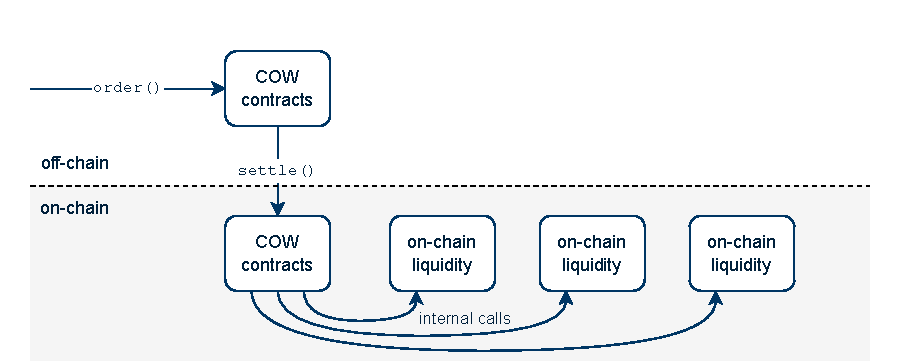
\includegraphics[width=\textwidth * \real{0.8}]{diagrams/cow2.pdf}
    \caption{CoW procotol execution. CoW services accumulate orders and batches are settled (at most) every 30 seconds.}
  \end{center}
\end{figure}

An AMM whose quote depends on the UCP of the CoW batch auction needs to have at least the following structures:
\begin{itemize}
  \item A way for traders to submit orders.
  \item A way for would-be LPs to add or remove liquidity.
  \item A communication channel $\mathcal{O}$ connecting Feedlot with the CoW contracts or services along which can be communicated the UCP.
\end{itemize}
Since the last item is the distinguishing feature of Feedlot AMMs, in this section we focus on the design of this channel.

\subsection{Synchronisation}

A batch auction system needn't be synchronised with the blockchain.
%
There may not be an auction every block, and even if there is, not every token pair traded on the BAS need necessarily appear in the batch.
%
This is the case for CoW: auctions are roughly every 30 seconds, and sometimes no auction occurs for hours at a time.
%
Therefore, a fresh batch auction price might not be available at the point that a trader wishes to trade on feedlot.

If the Feedlot quote price is to depend on the price of a CoW batch auction, then, there are only two possibilities:
\begin{enumerate}
  \item The quote function uses a stale CoW price (poll model).
  \item The market only settles trades at the same time as the batch auction (subscription model).
\end{enumerate}
These two options are analogous to what in the blockchain oracles literature have been called the \emph{pull} and \emph{push} models, respectively \cite{heiss2019oracles,muhlberger2020foundational}.

In either case, CoW services can guarantee zero latency updates of the UCP by writing into the channel atomically together with the batch execution transaction. 
%
This would require minor modifications to CoW's offchain components so that they call a wrapper contract that both triggers the CoW settlement and publishes a price to the on-chain oracle.
%
It does not require any changes to CoW's onchain components.
%
\begin{figure}
  \begin{center}
    \vspace{2ex}
    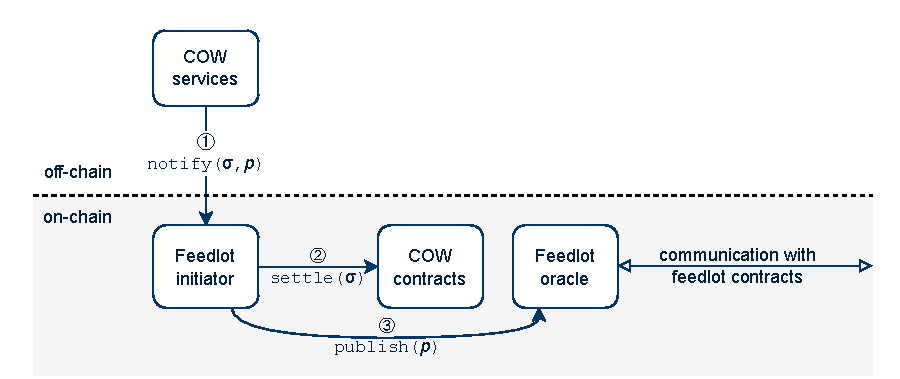
\includegraphics[width=\textwidth * \real{0.8}]{diagrams/wrapper.pdf}
    \caption{Atomic execution of the batch solution and publication of the UCP. The ordering of (2) and (3) can be reversed.}
  \end{center}
\end{figure}
%
Whether the UCP is updated before or after the settlement affects only how Feedlot behaves for orders placed in the winning solution itself, with the details depending on the synchrony model for Feedlot; see \S\ref{solution-on-feedlot}.
%
Orders that arrive at Feedlot outside the batch are not affected by this ordering.

What could be considered a third option is to fall back on another algorithm in case no price is available. 
%
Since that essentially amounts to not trading on Feedlot, and could easily be implemented at a higher layer, we don't discuss that here.

\subsubsection{Poll model}

In this model, CoW writes the UCP vector to the channel every time there is a batch. Meanwhile, Feedlot AMMs query the price whenever they have to settle an order.
%
There is no synchronisation between these two tasks.
%
One write is needed per batch per product, and one read is needed per trade on Feedlot.
%
These operations being relatively cheap, it would be reasonable to implement this type of channel as an on-chain oracle.
%
\begin{figure}
  \begin{center}
    \vspace{1ex}
    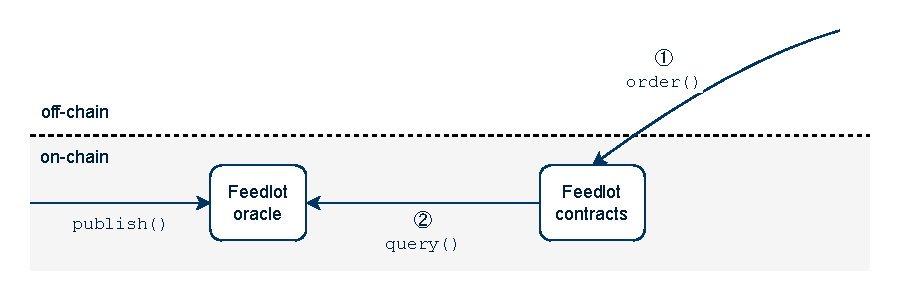
\includegraphics[width=\textwidth * \real{0.8}]{diagrams/poll.pdf}
    \caption{Polling oracle. Feedlot AMM executions are not synchronised with CoW batches.}
  \end{center}
\end{figure}
%
A variant approach is to aggregate UCPs to produce, for example, time-weighted average prices. This is the approach taken by Uniswap's oracle service \cite{adams2020uniswap}.

\subsubsection{Subscription model}

In this approach, orders arriving at Feedlot are accumulated in an order book.
%
All trades are executed when there is a CoW batch.
\begin{figure}
  \begin{center}
    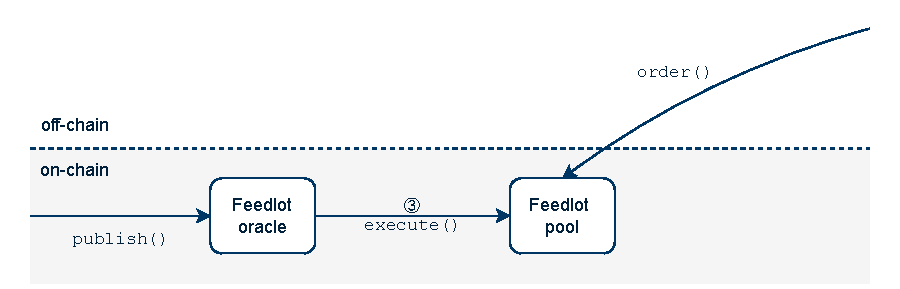
\includegraphics{diagrams/sub.pdf}
    \caption{Subscription oracle. Feedlot AMM executions are triggered when a new price is published.}
  \end{center}
\end{figure}

As with any order book based protocol, the order book itself would potentially be quite expensive to maintain on the Ethereum chain.
%
It is beyond the scope of this report to discuss approaches for optimising trust model and cost-effectiveness of off-chain order books.
%
Pragmatically, a reasonable approach would be to maintain the order book in the same place as the order book for the CoW batch auction, which at time of writing is a set of servers maintained by the CoW team.
\begin{figure}
  \begin{center}
    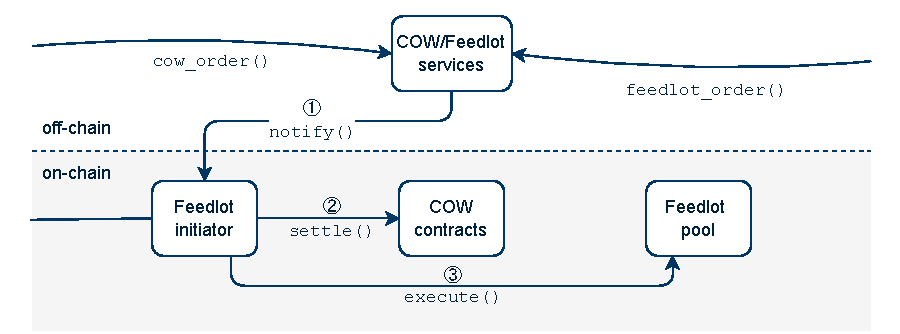
\includegraphics{diagrams/sub-merged.pdf}
    \caption{Integrated oracle with offchain order queue. Feedlot AMM executions are triggered when a new price is published.}
  \end{center}
\end{figure}

\subsection{Can the batch itself settle on Feedlot?}
\label{solution-on-feedlot}

Certain configurations would allow the solution to both settle orders on Feedlot and quote it a price.
%
The solver's objective is to get the most favourable price possible for its users, so naturally it will quote the least favourable price that Feedlot will accept.
%
Naturally, allowing an entity to trade against the AMM at any price it chooses is trivially exploitable to the detriment of LPs, and so special care has to be taken to address this case.


\subsubsection{Poll model}

In the poll-based model, 
\begin{itemize}
  \item If the UCP is updated \emph{after} the batch, the solution trades with a stale price.
  \item If the UCP is updated \emph{before} the batch, the solution trades at the price quoted by the solver.
\end{itemize}
The interesting case is the second one. 
%
Assuming solutions are simulated exactly as they would run on-chain, a solver could quote any price at all and have it execute successfully against Feedlot.
%
The solver's objective is to get the most favourable price possible for its users, so naturally it will quote the least favourable price that Feedlot will accept.
%
Naturally, allowing an entity to trade against the AMM at any price it chooses is trivially exploitable to the detriment of LPs.
%
Thus, if this approach were to be pursued, a special mechanism would have to implemented where Feedlot is specifically excluded from simulation.

Let us discuss, and dismiss, in turn a few approaches to making this work:
\begin{itemize}
  \item 
    Bound Feedlot's pricing function below independently of the UCP. For example, accept a trade only if it offers better pricing for the pool than some hardcoded aggregate of prices from whitelisted external markets.
    %
    Then rational solvers will always trade at exactly this lower bound.
    %
    This eliminates the dependence of pricing on the UCP.
    
  \item
    Adjust the solution objective to some strictly convex function that takes into account utility of the pool as well as active traders.\footnote{If it isn't \emph{strictly} convex, solvers will be indifferent between delivering utility to traders or the pool.}
    %
    The objective function will have to be normalised so that, independently of absolute price, it achieves some desired balance between pool and trader utility.
    %
    Clearly, this price normalisation cannot be derived from the price quoted by solvers, because as before they would then be free to set it arbitrarily.
    %
    Hence, an auxiliary price oracle is needed.
    
  \item
    Allow solutions that successfully simulate on markets other than Feedlot to actually settle instead on Feedlot, at the price that was realisable on those markets.
    %
    This has the effect of making price manipulation costless: solvers can provide their own liquidity at any price, knowing that they will not be held to trading at that price, this burden ultimately falling on Feedlot LPs.
    
\end{itemize}
It is possible that some combination of these and other approaches could allow solvers to safely both trade and quote on the Feedlot liquidity pool.


\subsubsection{Subscription model}

Batch solutions must settle immediately, so the success of the solution cannot depend on trading on an AMM that enqueues orders for execution at a later time.
%
However, a batch can be used to atomically execute any message call.
%
A solver could therefore use the following strategy:
\begin{enumerate}
  \item Fill orders using private liquidity.
  \item Enqueue orders in the opposite direction on Feedlot.
\end{enumerate}
Financially, this amounts to hedging the trade in step 1.~with a forward contract with expiry at the next batch.
%
In this way, Feedlot could act as a kind of repo market for solvers.

\section{Cryptoeconomic security}
\label{security}

A price oracle is a data source $\oracle$ from which a smart contract may query prices for a market order 
\[
  p \leftarrow \oracle (t_\mathrm{in},t_\mathrm{out},\sigma,r)
\]
where $t_\mathrm{in/out}$ denotes the in/out token, $\sigma\in\{\mathrm{BUY},\mathrm{SELL}\}$ is the direction, and $r$ is the amount (of $t_\mathrm{in}$ for SELL orders, $t_\mathrm{out}$ for BUYs).
%
The oracle is said to be \emph{truthful} if the prices thereby obtained are free from arbitrage.

Assuming correct implementation, oracles can fail in two ways:
\begin{itemize}
  \item Inaccurate or unreliable data source.
  \item Failure to faithfully communicate the value from the data source.
\end{itemize}
In the present context, fidelity of the communication of value is guaranteed by non-falsifiability of on-chain execution.

\subsection{Truthfulness of pricing data}
\label{realisable}

We say that the price $p$ is \emph{realisable} for an agent $I$ at a volume $V$ of the in token and chain state $\phi$ if it is possible for $I$ to buy $V$ $A$ tokens for $pV$ $B$ tokens in state $\phi$.
%
This is a way to make sense of the `truthfulness' property for oracles sketched in \cite{heiss2019oracles}.

If CoW solver prices are not realisable, the solver must settle the trade with their own private liquidity held in bond by CoW DAO.
%
A posteriori, CoW solver prices are realisable for the solver at the state immediately before the batch and at the volume traded in the batch.
%
That is, the structure of the CoW batch auction itself guarantees that the UCP vector is realisable at the volume traded in the batch.

It is worth noting that merely simulating executions on-chain (and reverting all changes at the end) is sufficient to verify realisability of the price vector.

\subsection{Manipulation resistance}
\label{manipulation}

Wherever economic decisions are made based on the output of an oracle $\mathcal{O}$, there lies an incentive to effect changes in the value published by $\mathcal{O}$ in order to influence those decisions. 
%
In few settings is this incentive more transparent than the present case of a price oracle coupled with an automated market that offers to trade at or near that price.
%
If, for example, some party is able to manipulate $\mathcal{O}$ at a cost $C_\mathrm{manip}$ so that it publishes a price $p$ that is strictly less than a price $p_\mathrm{ext}$ realisable on some other market, then a strategy of doing so and then buying a quantity $V$ of the risky asset on Feedlot yields a profit of
\[
  V\cdot (p_\mathrm{ext}-p) - C_\mathrm{manip}.
\]
Even if this quantity is negative, trading on Feedlot in this way \emph{offsets} the cost of manipulation, which may still be strategically optimal because of other decisions contingent on the output of $\oracle$.
%
Note that this type of activity does not undermine the fidelity of the oracle itself: a manipulated price may still be realisable.

In general, it is difficult to distinguish price manipulation from other types of economic activity that affects prices \cite{kyle2008define, zhang2022competition}.
%
However, it is quite straightforward to define \textbf{manipulation resistance}, at least at an intuitive level: a trading game whose payoffs depend on a parameter $p$ is $p$-manipulation resistant if the cost of effecting a change in $p$ away from its `natural' value is greater than the marginal profit that can be made by exploiting such a price change:
%
\[
  C_\mathrm{manip}(V,p,p_\mathrm{ext}) \gg U(\sigma;p) - U(\sigma';p_\mathrm{ext}).
\]
Here $\sigma$ is a strategy that is optimal at oracle price $p$ and $\sigma'$ is an optimal strategy at oracle price $p_\mathrm{ext}$.

To analyse this property concretely, it is necessary to have models for the strategy space.
\begin{itemize}
  \item 
    To cause the CoW UCP to be equal to $p<p_\mathrm{ext}$ at volume $V_\mathrm{CoW}$, it is necessary and sufficient to make available a volume $V_\mathrm{CoW}$ of the risky asset for purchase by a solver at price $p$.
    %
    Ignoring second-order effects such as the reaction of other market participants to a price change, the basic cost of this is given by
    \begin{equation}
    \label{cost-of-manipulation}
      V'_\mathrm{CoW}\cdot |p_\mathrm{ext}-p|,
    \end{equation}
    where $V'_\mathrm{CoW}\leq V_\mathrm{CoW}$ is the volume of user orders in the batch not placed by the manipulator.
    
  \item 
    To model the marginal proceeds of manipulation, we consider only the direct profits from trading on Feedlot at favourable prices, that is,
    \[
      V_\mathrm{Feedlot}\cdot\left|p-p_\mathrm{ext}\right|
    \]
    where $V_\mathrm{Feedlot}$ is the amount traded.
    %
    Other profits from as-yet unrealised uses of $\oracle$ are difficult to predict.
    %
    CoW or would-be Feedlot developers may have some ability to constrain, or at least channel, decision-making based on $\oracle$ by restricting on-chain access.
    %
    However, the feed would still be visible to anyone with access to an Ethereum node.
    
\end{itemize}
With these models, the essential condition for manipulation resistance is
\[
  V_\mathrm{Feedlot} < V'_\mathrm{CoW}.
\]
If $V'_\mathrm{CoW}$ can be estimated, this inequality can be enforced in the form of a volume limit for Feedlot.
%
Unfortunately, it is hard to calculate $V'$ in practice, because orders owned by an agent following a manipulation strategy cannot easily be distinguished from the orders of other agents.
%
The potential for low-cost wash trading means that in general, it need not be possible to estimate $V'$ in terms of $V$.

\section{Economic impact}

\subsection{For LPs}
In \S\ref{price-feed}, we characterised the introduction of a price feed to our AMM pricing function as a way to mitigate or prevent LP losses due to adverse selection.
%
Can we quantify the effects of this mitigation in practice?

In \cite{milionis2022automated}, the authors introduce a framework to quantify losses of CFMM LPs to adverse selection that depends on an external market price $P$.
%
Adapting this framework to discrete time and with the CoW UCP playing the r\^ole of the external market price, we can define the \emph{CoW-based loss-versus-rebalancing} as
\[
  \mathrm{LVR}_n \defeq R(P_n) - V(P_n)
\]
where:
\begin{itemize}
  \item $P_n$ is the UCP of the $n$th CoW batch;
  \item $V(P_n)$ is the optimal CFMM pool value at an external market price of $P_n$;
  \item 
    $R(P_n) = V_0 + \sum_{i=1}^n y^*(P_n)\cdot (P_n-P_{n-1})$ is the value of the self-financing rebalancing portfolio at the time of the $n$th CoW batch, where rebalances take place only at CoW batch times.
    %
    (If trading fees are negligible, path-independence means that it doesn't actually matter when rebalancing takes place.)
    
\end{itemize}
Discrete-time analogues of the arguments of \emph{op.~cit}.~show that this is a non-negative and non-decreasing process.\footnote{We lose the predictability property, because of course, the discrete-time analogue of a diffusion process is not predictable.} 
%
In continuous time, the quantity can be expressed in terms of the instantaneous square volatility $\sigma^2(P)$ and $V''(P)>0$; one can derive similar, though uglier, formulas for the discrete case.

If Feedlot uses passthrough pricing and accepts trades in such a way that its reserves track the rebalancing portfolio, then $R_n$ can also be interpreted as the portfolio value of a Feedlot LP.
%
That is, $\mathrm{LVR}_n$ is the difference in performance between a Feedlot LP and a CFMM LP.
%
This is contingent on a sufficient `uninformed' order flow arriving at Feedlot for it to track the reference portfolio by selectively accepting trades.

\

\begin{center}[DATA STUDIES GO HERE]\end{center}

\subsection{For traders}

Feedlot LPs take up a short position on a kind of option to trade at a certain oracle price. 
%
But by construction, this price is also realisable on other markets; that is, this optionality already exists `naturally.'
%
Why then should traders be interested in purchasing this product?

\begin{itemize}
  \item 
    \emph{Protection.} By trading along with the CoW batch, the risk of price changes between commitment and execution time (whether due to `natural' variability or deliberate attack) is socialised across the whole CoW/Feedlot execution.
    %
    Traders on CoW itself also enjoy this benefit.
    
  \item
    \emph{Spread}. User orders on the CoW batch auction employ solvers to actively seek out favourable prices. On the other hand, market orders on Feedlot simply wait for someone on CoW to ask for a price for that pair and then take advantage of the result.
    %
    Feedlot LPs do no price-finding work, and depending on how the liquidity curve is configured, may also enjoy portfolio management services (at the cost of unpredictable execution prices for users).
    %
    Hence, Feedlot trading fees (or equivalently, the bid-ask spread) must be cheaper than the active service provided by CoW protocol.

\end{itemize}

\section{Conclusion}

A safe implementation of a Feedlot AMM on the subscription model would provide traders with cheap trading at up-to-date instantaneous market prices.
%
Unlike traditional static CFMMs, Feedlot protects LPs from adverse selection, while still offering an option to enjoy flexibly priced portfolio management. 
%
It would also yield a new revenue stream for CoW protocol in the form of oracle fees.

The question of whether a safe implementation is possible requires further research.
%
A team wishing to implement a Feedlot AMM must take great care to ensure that it does not make the CoW UCP an economically viable target for manipulation, inviting harm on Feedlot LPs and users and stakeholders of CoW protocol alike.
%
In \S\ref{manipulation}, we have established that some kind of volume controls are a necessary condition for manipulation resistance.
%
However, na\"ively limiting volume in terms of the volume on CoW is not sufficient, since this quantity is itself prone to relatively low-cost manipulation.
%
Furthermore, if the scale of traditional derivative markets is anything to go by, there is likely to be interest in increasing the allowable volume to possibly as much as several times the volume of the CoW batch itself.

We propose three basic avenues of investigation
\begin{itemize}
  \item
    \emph{Visibility.}
    Efforts should be made to make manipulation \emph{detectable} if it occurs.
    %
    There are a number of immediate difficulties with this endeavour:
    \begin{itemize}
      \item 
        It is not straightforward to even define the notion of manipulation. Widely acknowledged is the necessary component of \emph{intent}. we also need to be able to make sense of the `non-manipulated' price, for which we need insight
      \item 
        In pseudonymous blockchain environments, identities are by default not Sybil-resistant. It is not generally possible to prove that two addresses acted in concert, which would be.
        %
        This problem could be mitigated by the adoption of a Sybil-resistant authentication system as a requirement for using CoW swap and Feedlot.
      \end{itemize}

  \item
    \emph{Make manipulation more expensive.}
    If a manipulator can reliably effect atomic execution of his manipulation strategy with the CoW/Feedlot batch, then the cost to manipulate is given by the expression (\ref{cost-of-manipulation}).
    %
    The only actor who can achieve atomicity with certainty is the solver itself.
    
  \item
    \emph{Constrain the marginal proceeds of manipulation.}
    
    
  \item
    \emph{Control solver activities.}
    Solvers, as the most privileged actors in the CoW ecosystem, are inherently particularly resistant to the mitigation heuristics heretofore discussed.
    %
    On the other hand, a solver has a Sybil-resistant identity and economic exposure to the CoW DAO in the form of his bond.
    %
    Moreover, the CoW DAO has a direct channel to influence the incentive structure of solvers via the batch auction objective function.
  
\end{itemize}

    \emph{Social enforcement.} 
    The solver itself is the most privileged actor in this game. 
    %
    While this places it in a uniquely powerful position to manipulate CoW prices itself --- and therefore ought to be the subject of particular scrutiny --- it also is uniquely positioned to fight \emph{against} manipulation by arbitraging manipulated prices into line with external markets in its solution.
    %
    However, fighting against manipulation is not necessarily aligned with the objective function currently in effect on CoW protocol.
    %
    As it stands, CoW solvers are already economically exposed to the governance decisions of the CoW DAO.


\begin{example}
In some cases, trading against a would-be manipulator may be economically viable even without social enforcement.
%
Suppose a wash trader submits a large volume of liquidity orders in both directions.
%
Suspecting a manipulation attempt, the solver discards the orders in one direction and himself takes the opportunity to make a large directional trade with no slippage.
\end{example}

\printbibliography
\end{document}
